% Titre : Equation à paramètre
% Filiere : BCPST
% Difficulte :
% Type : DS, DM
% Categories : analyse
% Subcategories : 
% Keywords : analyse




\vspace{0.5cm}
\begin{exercice}
%\paragraph{Exercice 2 : Equation à paramètre} 
On note $\Delta(m) =m^2-8m+12$.  
\begin{enumerate}
\item Résoudre l'inéquation d'inconnue $m$: 
\begin{equation}\tag{$I_1$}
\Delta(m)>0
\end{equation}
\item On note $r_+(m) =\frac{m+\sqrt{\Delta(m)}}{4}$ et $r_-(m) =\frac{m-\sqrt{\Delta(m)}}{4}$.\\
%Quel est le domaine de définition de $r_+$ et $r_-$ ? 
\item Résoudre 
$$r_+(m)\geq 1 \quad \text{ et } \quad r_-(m)\geq 1 .$$
\item  Résoudre l'inéquation d'inconnue $y$ et de paramétre $m\in \R$
\begin{equation}\tag{$I_2$}
  \frac{2y^2-\frac{3}{2}}{y-1}\geq m
\end{equation}
\end{enumerate}
\end{exercice}


\begin{correction}
\begin{enumerate}
\item Le discriminant réduit de $\Delta(m)$ vaut $\delta(m) = 16-12=4.$ Les racines de $\delta(m)$ valent  donc $m_1= 4-2=2$ et $m_2=4+2=6$. Donc $\Delta(m) =(m-2)(m-6)$ et 
les solutions de $\Delta(m)>0$ sont
$$\cS = ]-\infty, 2[\cup ] 6,+\infty[.$$

\item Les expressions $r_+(m)$ et $r_-(m)$ sont définies pour $\Delta(m) \geq 0$ soit 
$m\in  ]-\infty, 2]\cup [ 6,+\infty[.$

Résolvons $r_+(m) \geq 1$  pour $ m \in  ]-\infty, 2]\cup [ 6,+\infty[.$
\begin{align*}
& \frac{m+\sqrt{\Delta(m)}}{4} \geq 1\\
\Longleftrightarrow\quad  & m+\sqrt{\Delta(m)} \geq  4 \\
\Longleftrightarrow\quad  & \sqrt{\Delta(m)} \geq  4 -m\\
\end{align*}
Si \underline{$(4-m) <0$}, $m$  est solution car $\sqrt{\Delta(m)} \geq 0$.\\

Si \underline{$(4-m)\geq 0$}, l'équation $r_+(m) \geq 1$  est équivalente à 
\begin{align*}
&\Delta(m) \geq (4-m)^2\\
\Longleftrightarrow\quad  & m^2-8m+12 \geq m^2 -8m +16 \\
\Longleftrightarrow\quad  & 0 \geq 4
\end{align*}
Donc pour tout $m\leq4$, $m$  n'est pas solution. 

Finalement, les solutions de $r_+(m) \geq 1$ sont 
$$\cS_+ = [ 6,+\infty[.$$



Résolvons $r_-(m) \geq 1$  pour $ m \in  ]-\infty, 2]\cup [ 6,+\infty[.$
\begin{align*}
& \frac{m-\sqrt{\Delta(m)}}{4} \geq 1\\
\Longleftrightarrow\quad  & m-\sqrt{\Delta(m)} \geq  4 \\
\Longleftrightarrow\quad  & m-4 \geq   \sqrt{\Delta(m)} \\
\end{align*}
Si \underline{$(m-4) <0$}, $m$  n'est  pas solution car $\sqrt{\Delta(m)} \geq 0$.\\

Si \underline{$(m-4)\geq 0$}, l'équation $r_-(m) \geq 1$  est équivalente à 
\begin{align*}
& (m-4)^2\geq \Delta(m) \\
\Longleftrightarrow\quad  & m^2-8m+16 \geq m^2 -8m +12 \\
\Longleftrightarrow\quad  & 4 \geq 0
\end{align*}
Donc pour tout $m\geq 4$, $m$  est  solution. 

Finalement, les solutions de $r_-(m) \geq 1$ sont 
$$\cS_+ = [ 6,+\infty[.$$


\item L'ensemble de définition de  $ \frac{2y^2-\frac{3}{2}}{y-1}$ est $D_1 =\R\setminus\{  1\}$. 
On va résoudre \begin{equation}\tag{$I_4(m)$}
 \frac{2y^2-\frac{3}{2}}{y-1}\geq m
\end{equation}
en fonction de $m\in \R$.\\

Pour tout $y \in D_1$  on a 
\begin{align*}
  \frac{2y^2-\frac{3}{2}}{y-1}- \frac{m(y-1)}{y-1}\geq  0\\
    \frac{2y^2-\frac{3}{2} -m(y-1)}{y-1}\geq  0\\
        \frac{2y^2-my + (-\frac{3}{2} +m)}{y-1}\geq  0\\
\end{align*}

Le discriminant de $2y^2-my + (\frac{3}{2} +m)$ vaut 
$$m^2 -4(2) (-\frac{3}{2} +m) = m^2 -8m +12.$$
On reconnait l'expression de $\Delta(m)$. 

\begin{enumerate}
\item D'après la question $1$,  $\Delta(m) >0 $ pour $m \in  ]-\infty, 2[\cup ] 6,+\infty[$. Sur cet ensemble le polynôme $2y^2-my + (-\frac{3}{2} +m) $ admet deux racines, $r_-(m)$ et $r_+(m)$. Donc 
$$2y^2-my + (-\frac{3}{2} +m)  = 2 ( y-r_-(m) ) (y-r_+(m)).$$

Pour $m\geq 6$, d'après la question $2$, on a :
$$r_+(m) \geq r_-(m) \geq 1 $$

\end{enumerate}
On note $q(y)=2y^2-my + (-\frac{3}{2} +m) $
\begin{tikzpicture}
   \tkzTabInit{$y$ / 1 , $ q(y) $/1 , $y-1$/ 1, $\frac{q(y)}{y-1}$/ 1.5}{ $-\infty$ , $1$, $r_-(m)$, $r_+(m)$, $+\infty$}
   \tkzTabLine{, +, , +,z,- ,z, +, }
  \tkzTabLine{, -, z, +,,+ ,, +,  }
    \tkzTabLine{, -,, +,z,- ,z, +,  }
  
\end{tikzpicture}

Les solutions de l'équation $I_4(m)$ pour $m \geq 6$  sont 
\begin{center}
\fbox{ $S =]1,r_-(m)]\cup [r_+(m), +\infty[$ }
\end{center}
Pour $m\leq 2$, d'après la question $2$,  on a :
$$1\geq r_+(m) \geq r_-(m) $$
%
%
\begin{tikzpicture}
   \tkzTabInit{$y$ / 1 , $ q(y) $/1 , $y-1$/ 1,  $\frac{q(y)}{y-1}$/ 1.5}{ $-\infty$ ,  $r_-(m)$, $r_+(m)$, $1$, $+\infty$}
   \tkzTabLine{, +, z, -,z,+ ,, +, }
  \tkzTabLine{, -, , -,,- ,, +,  }
      \tkzTabLine{, -,z, +,z,- ,, +,  }
\end{tikzpicture}
Les solutions de l'équation $I_4(m)$ pour $m \leq 2$  sont 
\begin{center}
\fbox{ $ S =[r_-(m),r_+(m)]\cup ]1, +\infty[.$ }
\end{center}
\item Pour $\Delta(m) =0 $, c'est-à-dire  $m \in { 2,6}$. 
Pour $m=2$, on a $r_+(2)=r_-(2) = \frac{1}{2}$ et 
$$2y^2-2 y +(-\frac{3}{2}+2) = 2 (y-\frac{1}{2})^2$$
et les solutions de $I_2$ sont donc 

\begin{center}
\fbox{ $ S=\{ \frac{1}{2}\} \cup ]1,+\infty[.$ }
\end{center}
Pour $m=6$, on a  $r_+(6)=r_-(6) = \frac{3}{2}$ et 
$$2y^2-6 y +(-\frac{3}{2}+6) = 2 (y-\frac{3}{2})^2$$
et les solutions de $I_2$ sont donc 
\begin{center}
\fbox{ $ S=]1,+\infty[.$ }
\end{center}


\item Pour $\Delta(m) <0 $, c'est-à-dire  $m \in ] 2,6[$. 

Le polynome $q$ n'a pas de racine réelle. Il est donc strictement positif  sur $\R$. Les solutions de $I_4(m)$ sont donc 
\begin{center}
\fbox{ $ S=]1,+\infty[.$ }
\end{center}

\end{enumerate}
\end{correction}